\section{数据质量统计}
使用Pacbio测序平台对A16R菌种进行测序。共得到4个smrtcells进行测序。
\subsection{质量统计方法}
Pacbio使用单分子测序技术实现高读长测序。但由于其数据信号捕捉困难,原始数据的质量较低,并且具有高随机性。因此,在数据分析前需要进行严格的数据质量过滤和前处理。
处理方法如下:
\begin{enumerate}
  \item 由于Pacbio使用环状文库进行测序,并且其实际读长远远大于文库长度。因此,大部分的原始数据可能被测了多次。因此,首先需要对原始数据进行打断和开环,并根据开环结果对测序数据的单个碱基进行一致性检验,并给出单碱基的质量值。
  \item 而后,使用严格的参数将残余的adapter进行去除。
  \item 最后,根据单碱基质量值,对reads中Q20<0.8的区域进行过滤和筛除,得到相对高质量的subreads序列进入后续分析。




\end{enumerate}



\subsection{测序数据质量统计结果}



\begin{figure}[H]

    \centering
    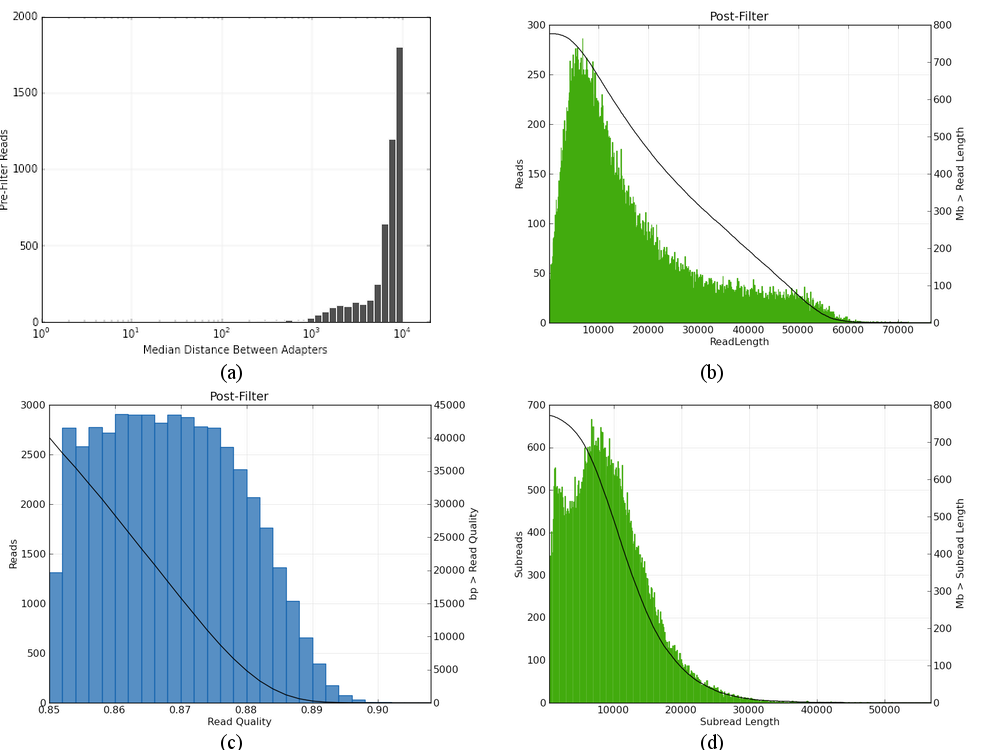
\includegraphics[width=0.8\textwidth]{qc.png}
    \captionsetup{labelsep=period}
    \caption{QC分析结果}
\end{figure}

\begin{enumerate}
    \renewcommand\theenumi{\alph{enumi}}
    \renewcommand\labelenumi{(\theenumi)}
      \item 测序得到的reads读长的统计图
      \item 下机原始数据的序列读长统计
      \item 经过数据过滤处理后得到的序列质量和数据量
      \item 经过数据过滤处理后得到的序列读长
\end{enumerate}





\subsection{所有测序结果统计表}
下表为测序结果的初步统计结果,其中,\textcolor{red}{红色数据}为经过数据质控后的可用数据的统计结果,后续分析全部使用这些质控后的数据进行分析。
\begin{table}[h]
    \caption{123}
        \begin{center}
            \begin{threeparttable}
                \begin{tabularx}{\textwidth}{cc|X}

                    \toprule
                    11&22&33\\
                    \midrule
                    aa&bb&静静地 \tnote{1} 我将离开你,请将眼角的泪逝去。漫漫岁月里\\

                    ee&ff&dd\\
                    \bottomrule

                \end{tabularx}
                \begin{tablenotes}

                    \footnotesize
                    \item[1] 我的天啊啊哪!!!
                \end{tablenotes}
            \end{threeparttable}
        \end{center}
\end{table}


